\question \textbf{Knapsack Problem}
Given the following instance of a Knapsack problem with 4 items with weight $w_i$ and value $v_i$. The knapsack capacity is 10. Model this problem as a graph problem to compute the subset of items with maximum total value fitting into the knapsack.

\begin{tabular}{c | c | c}
    $i$ & $w_i$ & $v_i$ \\
    \hline
    1 & 5 & 10 \\
    2 & 4 & 40 \\
    3 & 6 & 30 \\
    4 & 3 & 50
    \end{tabular}

\begin{solution}


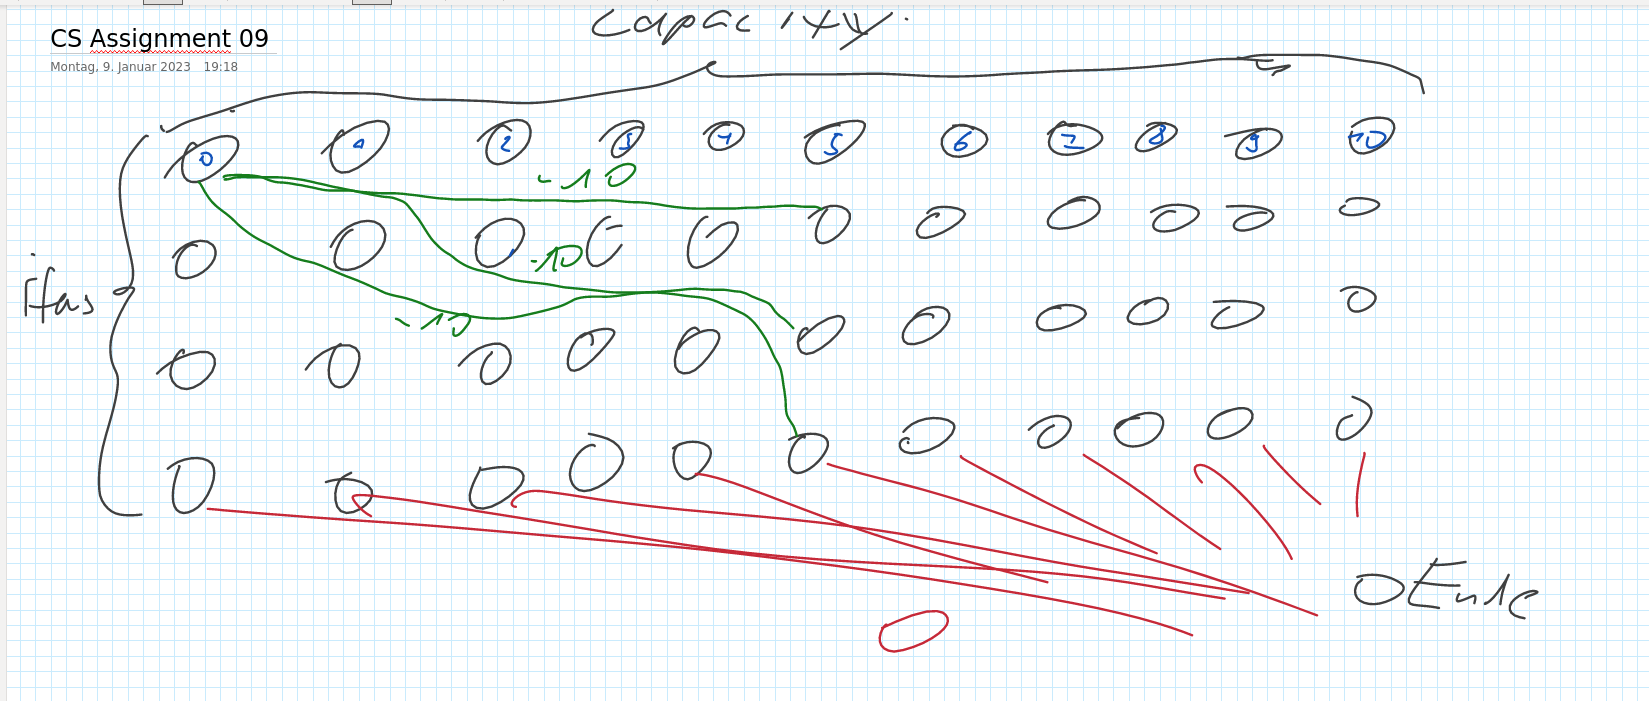
\includegraphics[width=0.8\linewidth]{task_5/Task_5.png}

As shown in the Graphic there is a grid like graph in which the cloumns represent the reached capacity and the rows represent the items.
If an item is chosen, we draw an edge to reached weight and label it with the negative value. From all nodes we also draw an edge reaching the end node with a value of 0.
We then calculate the shortest path using Bellman Ford. 


\end{solution}